

\section{Gaussian Mixture Models in R}

There are multiple packages for fitting mixture models in R.  We'll look at two -- |mixtools| and |MCLUST|.

\subsection{Installing mixtools}

The package |mixtools| can be installed via the GUI or the |install.packages| command. A \href{http://cran.r-project.org/web/packages/mixtools/vignettes/vignette.pdf}{mixtools vignette} can be downloaded from the CRAN website.

\subsection{Using mixtools}

We'll look at how to use mixtools using a data set on eruption times for the Old Faithful geyser in Yellowstone National Park (|?faithful| for details). We'll fit a univariate Gaussian mixture model to the time between eruptions data (\verb|faithful$waiting|).

\begin{R}
# allows us to refer to the variables within waiting time
# without using the standard list "$" syntax
> attach(faithful)

# create a nice histogram
> hist(waiting, main = "Time between Old Faithful eruptions",
xlab = "Minutes", ylab = "", cex.main = 1.5, cex.lab = 1.5, cex.axis = 1.4)

> library(mixtools)
> ?normalmixEM  # read the docs!
> wait.mix <- normalmixEM(waiting)

> names(wait.mix)
[1] "x"          "lambda"     "mu"         "sigma"      "loglik"     "posterior"
[7] "all.loglik" "restarts"   "ft"

# lambda is what we called "pi" in the lecture notes
> wait.mix[c("lambda","mu","sigma")]

> class(wait.mix)
[1] "mixEM"
> ?plot.mixEM  # read about the plotting options for the mixEM object
> plot(wait.mix, density=TRUE)
> plot(wait.mix, loglik=FALSE, density = TRUE, cex.axis = 1.4, cex.lab = 1.4, cex.main = 1.8, main2 = "Time between Old Faithful eruptions", xlab2 = "Minutes")
\end{R}


\begin{figure}[!ht]
    \centering
    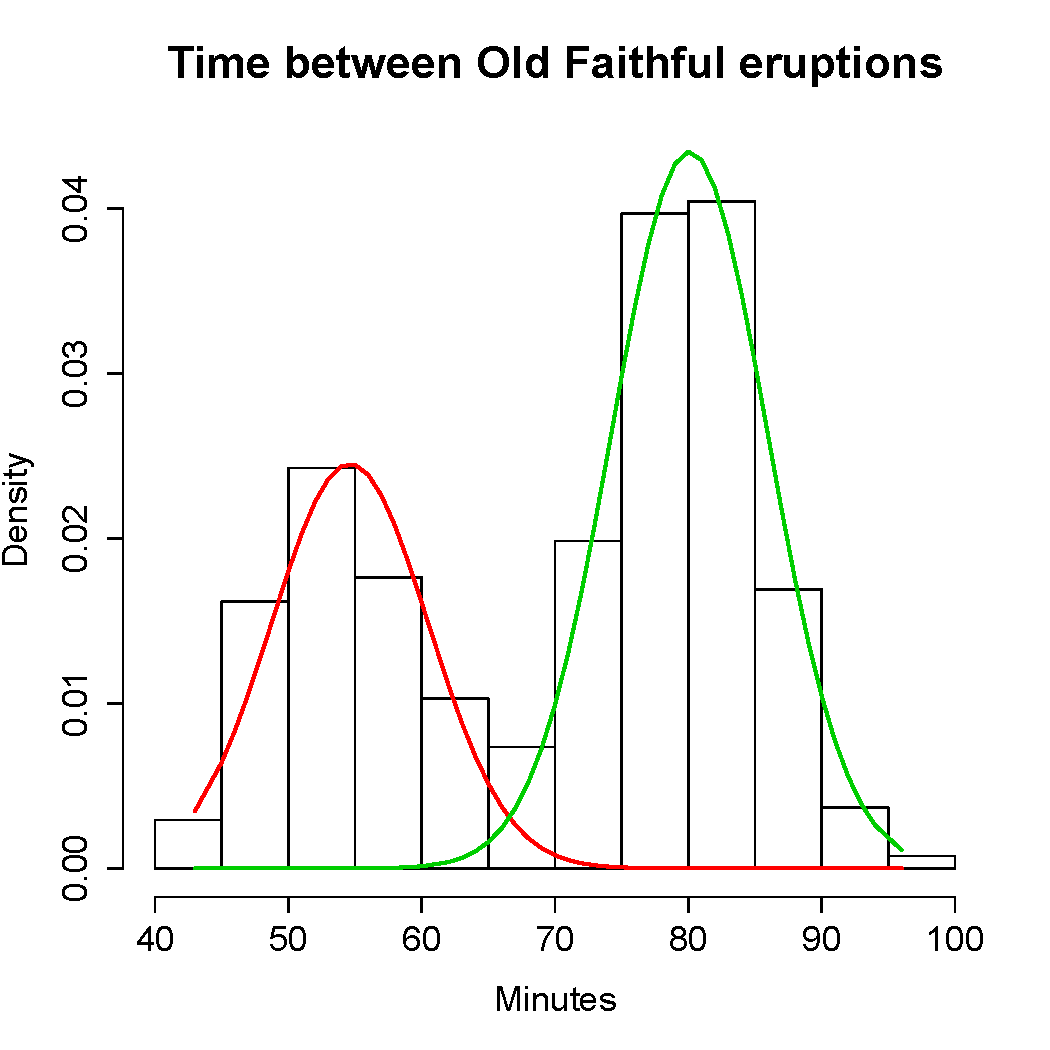
\includegraphics[width=0.5\columnwidth]{./figures/hands-on10/faithful-R.pdf}
    \caption{A Gaussian mixture model for the Old Faithful dataset, estimated using the mixtools module in R.}\label{fig:faithfulR}
\end{figure}


\subsection{Installing MCLUST}
The package |MCLUST| is one of another package that provides maximum likelihood based estimation of mixture models.  You will need to install the package (and it's dependencies) from the R GUI or using the |install.packages| command.

\subsection{Using MCLUST}

We're going to use two data set to illustrate some of |MCLUST|'s capabilities -- the iris data set we've worked with before, and the bivariate version of the Old Faithful data set. We'll start off with  the old faithful data set.

\begin{R}
> plot(faithful$eruptions, faithful$waiting)
\end{R}

From visual inspection of the bivariate scatter plot, it looks like there two clusters. Let's apply the |Mclust| function and see what it suggests:

\begin{R}
> library(mclust)
> fclust <- Mclust(faithful)
> fclust

 best model: elliposidal, equal variance with 3 components
\end{R}

Now that we've running the mixture model, let's look at the results graphically. The following call to |plot| will produce a series of plots.

\begin{R}
> plot(fclust)
\end{R}

The first plot gives is a diagnostic plot that shows the likelihood of the model as a function of  the number of groups (see BIC below). In general, when considering many possible models you want to pick the simplest model that has a highest likelihood. The second graphically represents the classification. The third plots highlights those objects for which the cluster assignment is most uncertain. The fourth plot gives a graphical representation of the Gaussian densities.

The |Mclust| function used a likelihood criterion called the ``Bayesian Information Criterion" (BIC) to estimate the number of components (clusters) in the mixture model. By this criterion it suggested 3 components. BIC, like other information criteria (the Akaike Information Criterion is another popular one), is designed to help choose among parametric models with different numbers of parameters. It tries to choose the simplest model that provides a good fit to the data.

\begin{R}
> names(fclust)
 [1] "modelName"      "n"              "d"              "G"              "BIC"
 [6] "bic"            "loglik"         "parameters"     "z"              "classification"
[11] "uncertainty"
> ?mclust  # check out the docs to read about all the returned parameters
\end{R}

Of course you don't have to accept the number of clusters that the |Mclust| function estimated. Here's how you'd calculate the mixture model with a user determined number of clusters:

\begin{R}
> fclust2 <- Mclust(faithful, G=2)
> plot(fclust2)
\end{R}

% Now let's generate some diagnostic plots for the mixture model:

% \begin{R}
% > plot(fclust)
% \end{R}

If you wanted to generate some of those plots individually you can do the following:

\begin{R}
# generate a plot showing the classifications predicted by mixture model
> mclust2Dplot(data = faithful, what = "classification", identify = TRUE,
    parameters = fclust$parameters, z = fclust$z)
\end{R}

See the docs for the |mclust2Dplot| function for other options.

\subsection{Mixture Models for the Iris data set}

The |MCLUST| package includes the function |clPairs|, a very nice extension of the |pairs| function, for creating scatter plot matrices with group information. The following code illustrates this:

\begin{R}
> names(iris) # remind yourself of the variables in the iris data set
[1] "Sepal.Length" "Sepal.Width"  "Petal.Length" "Petal.Width"  "Species"

# 5th variable is the Species classification
> clPairs(data=iris[,-5], classification=iris[,5])
\end{R}

\begin{figure}[!ht]
    \centering
    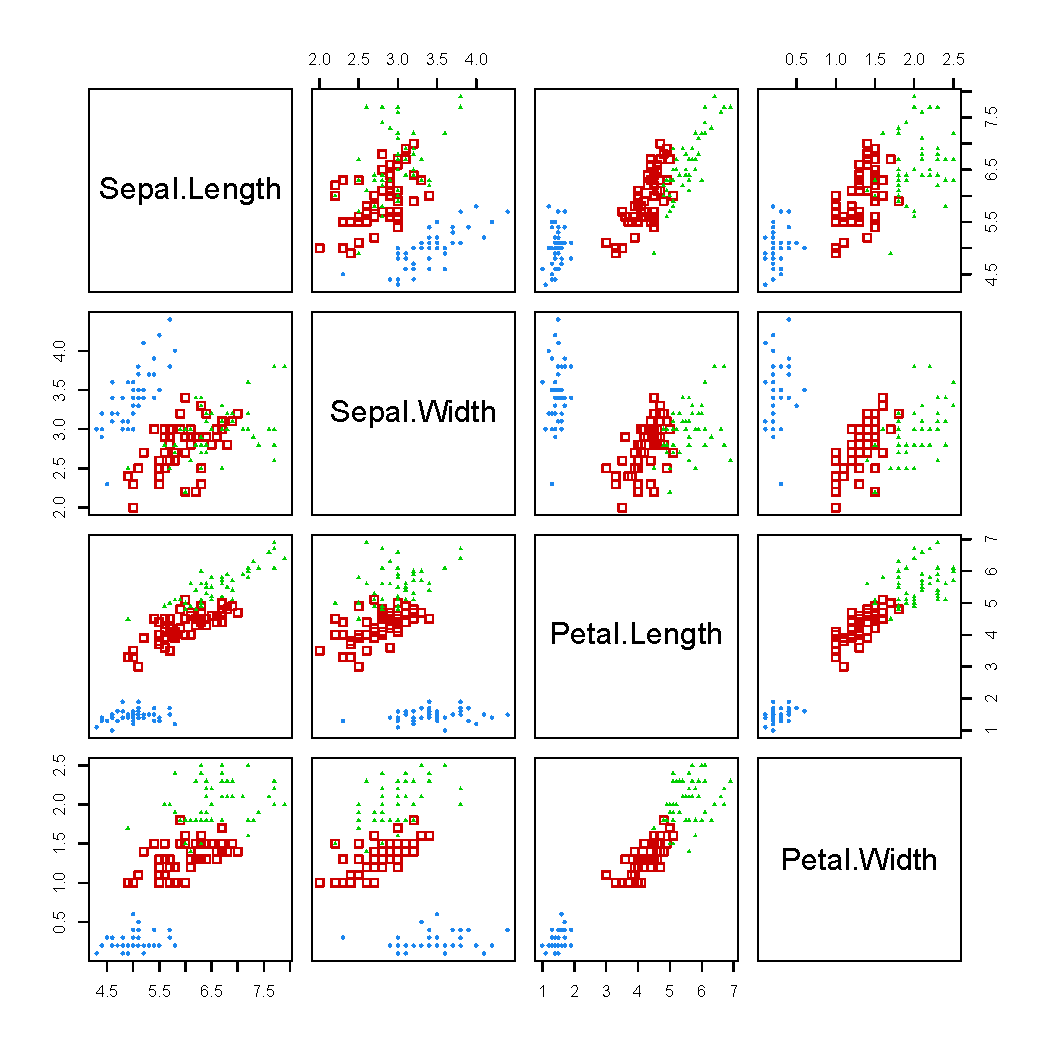
\includegraphics[width=0.5\columnwidth]{./figures/hands-on10/iris-clpairs.pdf}
    \caption{Output of the \texttt{clpairs} function for the iris data set.}\label{fig:clpairs}
\end{figure}

Let's see what |Mclust| makes of the iris data set:

\begin{R}
> iclust <- Mclust(iris[,-5])
> iclust

 best model: ellipsoidal, equal shape with 2 components
> plot(iclust)
\end{R}

Blind to the actual group structure the BIC suggests just two components, whereas we know there are three groups (though \textit{I. versicolor} is thought to be an allopolyploid hybrid; see Kim et al. (2007) Ann Bot, 100: 219-224. ). Examine the first graph produced by the |plot| call above to see how the 2 and 3 component models compare with respect to the BIC.

Now let's see how the mixture model does when we give it the true number of clusters:

\begin{R}
> iclust3 <- Mclust(iris[,-5], G=3)
> plot(iclust3)
\end{R}

To calculate the classification error rate we can compare the estimated clustering to the "true" (known) classification with the |classError| function (|?classError| for details):

\begin{R}
> classError(iclust3$classification, iris[,5])
$misclassified
[1] 69 71 73 78 84

$errorRate
[1] 0.03333333
\end{R}

The |uncerPlot| command allows us to visualize the uncertainty implied by the mixture model to see how uncertain the model was about the misclassified samples.

\begin{R}
> uncerPlot(iclust3$z, iris[,5])
\end{R}

In the uncertainty plot the vertical lines indicate the misclassified samples. As you can see those tend to be among the observations that the mixture model was most uncertain about with respect to which component they belonged to.


\subsection{More details on MCLUST}

See the \href{http://www.stat.washington.edu/research/reports/2006/tr504.pdf}{MCLUST docs} for in depth discussion of the use of |MCLUST|. The examples illustrated above were drawn from this documentation.


\subsection{Mixture Modeling in Python}

The package \href{http://scikit-learn.org/stable/}{scikit-learn} extends the SciPy library with a number of common machine learning algorithms, including an implementation of Gaussian mixture modeling.  |scikit-learn| is included with the EPD distribution you have already installed. The code below demonstrates how to use |scikit-learn| to carry out mixture modeling.

Before you get started use the the |write.table()| function in R to create a tab-delimited version of the |faithful| dataset (hint: use |"\t"| to specify tabs as the separator character, and dont include row names in the file). If you've properly formatted the file you should be able to open it as follows, and create a histogram:
%
\begin{python}
In [1]: f = np.loadtxt('faithful.txt', skiprows=1)
In [2]: f.shape
Out[2]: (272, 2)
\end{python}
%
Assuming that worked, let's import |scikit-learn| and fit a mixture model:
%
\begin{python}
In [4]: from sklearn import mixture
In [6]: classifier = mixture.GMM(n_components = 2)
In [7]: fit = classifier.fit(f[:,1])

In [22]: fit.means_  # means of the estimated subdistributions
Out[22]:
array([[ 80.12056513],
       [ 54.6623402 ]])

In [23]: fit.covars_  # (co)variances of the estimated substrituions
Out[23]:
array([[ 34.08969904],
       [ 34.95662279]])

In [66]: fit.weights_   #  weighting factors (pi in slides)
Out[66]: array([ 0.63770034,  0.36229966])

In [32]: x = linspace(40, 100, 200) # points at which to evaluate the model

# plot histogram using prob density rather than straight up frequency
In [33]: hist(f[:,1], normed=True, alpha=0.2, color='gray')

# draw the PDFs for the two estimated subdistributions
# notice how we multiply each normal PDF by it's weight

In [63]: plot(x, fit.weights_[0] * normpdf(x, fit.means_[0], sqrt(fit.covars_[0])),color='red')
In [64]: plot(x, fit.weights_[1] * normpdf(x, fit.means_[1], sqrt(fit.covars_[1])),color='blue')
In [73]: xlabel("Waiting Time")
In [74]: ylabel("Density")
In [75]: title("Time between Old Faithful eruptions")
\end{python}

\begin{figure}[!ht]
    \centering
    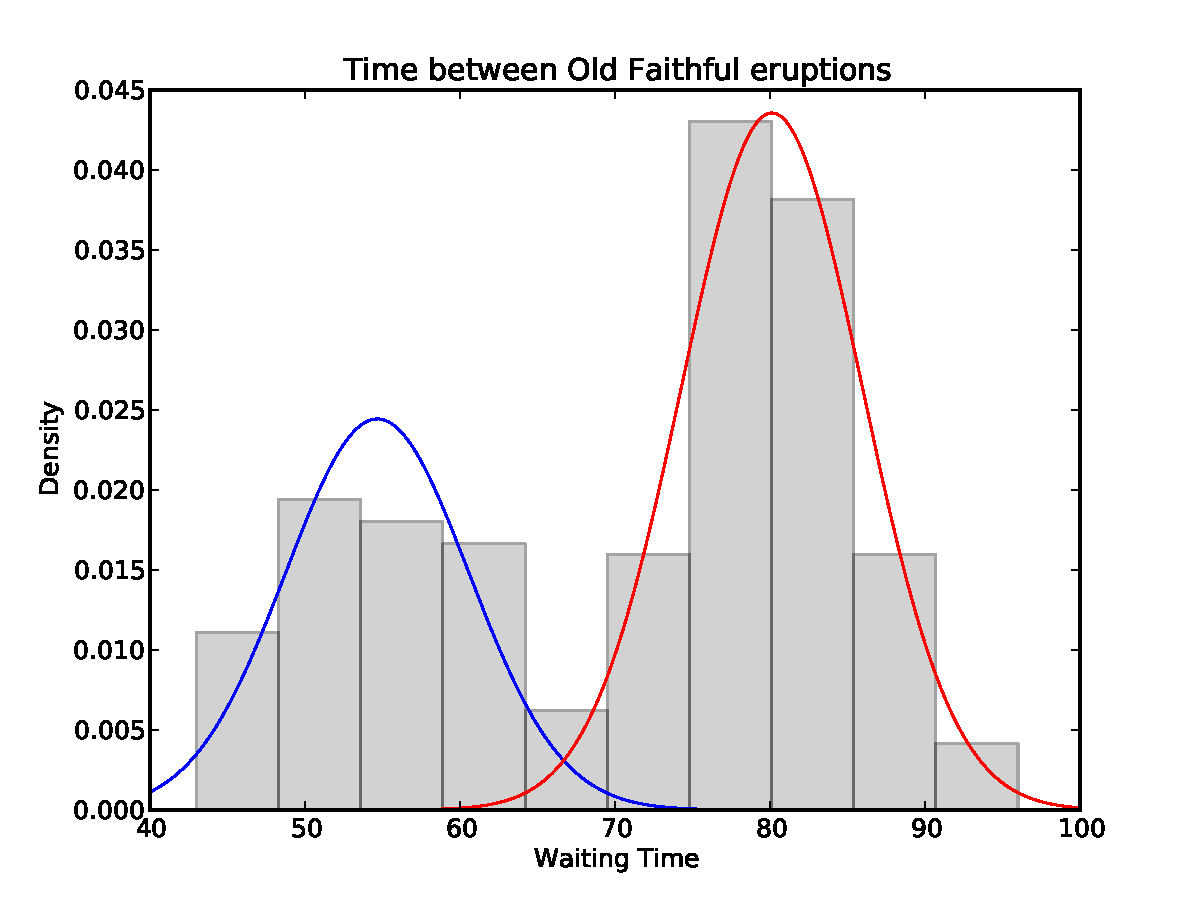
\includegraphics[width=0.5\columnwidth]{./figures/hands-on10/faithful-python.pdf}
    \caption{A Gaussian mixture model for the waiting time variable in the Old Faithful dataset, estimated using the scikit-learn module in Python.}\label{fig:faithfulpy}
\end{figure}

Now let's look at the binary data:
%
\begin{python}
In [4]: plot(f[:,0], f[:,1], 'k.')  # 'k.' gives small black dots as plot points
In [8]: xlabel("Eruption time (mins)")
In [9]: ylabel("Waiting time to next eruption (mins)")

# specify covariance_type = 'full' to estimate complete covariance matrices
In [10]: classifier2 = mixture.GMM(n_components=2, covariance_type='full')
In [11]: fit2 = classifier2.fit(f)

# setup grid to evaluate mixture model over
In [12]: x = linspace(1.5,5,200)
In [13]: y = linspace(40,100,100)
In [14]: X,Y = meshgrid(x, y)
In [23]: XY = np.c_[X.ravel(), Y.ravel()] # like R's c()

# evaluate the mixture model over the grid
In [24]: Z = log(-fit2.eval(XY)[0])
In [25]: Z = Z.reshape(X.shape)
In [26]: cntr = contour(X, Y, Z)
\end{python}
Check out the |scikit-learn| docs for more details and examples.

\begin{figure}[!ht]
    \centering
    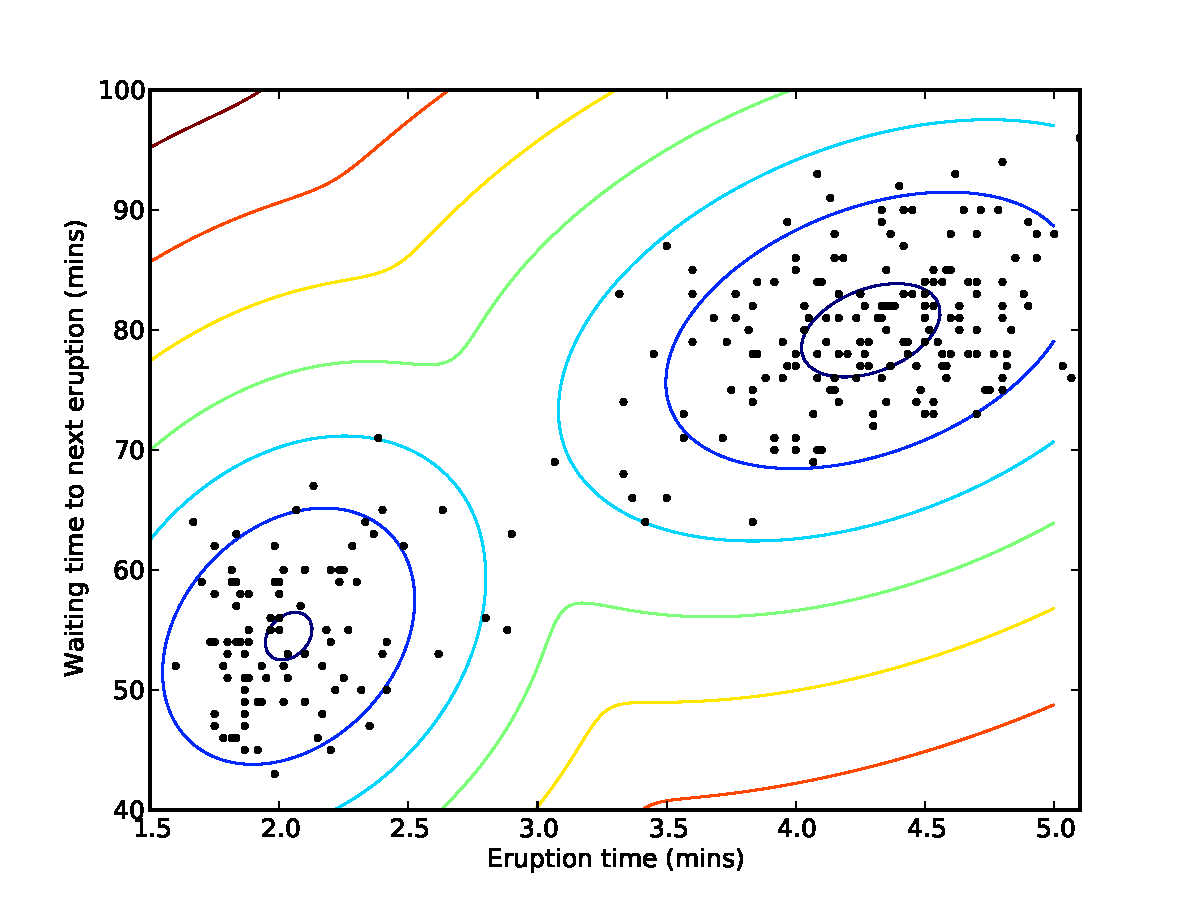
\includegraphics[width=0.5\columnwidth]{./figures/hands-on10/faithful2d-python.pdf}
    \caption{A Gaussian mixture model for 2D Old Faithful dataset, estimated using the scikit-learn module in Python.}\label{fig:faithfulpy2}
\end{figure}


\begin{assignment}
Download the dataset |ddata.txt| from the course wiki. This data set consists of 64 variables measured on 720 specimens. Use the various clustering and ordination techniques you've learned over the course of the semester to explore this data set and estimate the number of clusters in the data.  Use code and figures to support your conclusion.  Hint: you might consider using a lower dimensional approximation of the data to facilitate your analyses.

\end{assignment}


\section{Multidimensional scaling in R}

\subsection{Metric MDS}

The implementation of classic metric scaling in R is carried out using the |cmdscale()| function. Read the documentation for |cmdscale| and then work through the example showing the application of MDS to analysis of road distances between US cities available at the following link (but see notes below first):

\href{http://personality-project.org/r/mds.html}{http://personality-project.org/r/mds.html}.

\medskip
As you work through your example note the following:

\begin{itemize}
\item You can use the |source()| function not only with a local file but also with a URL.  This is convenient but potentially a security issue so don't run code willy nilly without checking out what it does.

\item You can download the code at \href{http://personality-project.org/r/useful.r}{http://personality-project.org/r/useful.r} and check out the functions that it includes. I thought the |read.clipboard()| function was particularly nice.
\end{itemize}





\subsection{Non-metric MDS}

The |isoMDS()| function in the |MASS| package implements the Shepard-Krusal version of non-metric scaling, while the |sammon()| function in the same package use the criterion proposed by Sammon (1969). You will need to utilize these functions, along with |cmdscale| and the hierarchical clustering functions covered last week for the following assignment.

\medskip
\begin{assignment}
Harding and Sokal (1998; PNAS 85:9370-9372; see course wiki) used cluster analysis and non-metric MDS to explore the relationship between European language families as measured by genetic distances among the people who speak those languages.  The classification they derived at large reflects geographic proximity but there are some language families that have distant genetic relationships to their geographic neighbors.

\medskip
Harding and Sokal provide a table of genetic distances that they used in their analyses. Use R to reconstruct the cluster analysis they report (Fig. 1) and repeat this analysis using neighbor joining. In a similar manner use both metric scaling and the Shepard-Kruskal and Sammon criteria for non-metric scaling to do an MDS analysis (similar to Harding and Sokal's fig. 2).  Try to also recreated the MST shown in their figure 2.

\medskip
Submit your code as an R markdown document, and include a brief paragraph describing what differences, if any, you found in your re-analysis of Harding and Sokal data. Are these differences significant (i.e. do they change your interpretation of the data)?

\end{assignment}



